\begin{figure}[t]
  \centering
  Full interior Gramian\\
  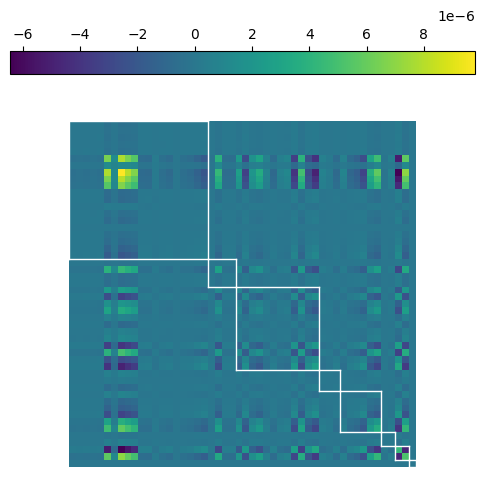
\includegraphics[width=0.43\linewidth]{kfac_pinns_exp/exp04_gramian_contributions/fig/gram_full.png}

  \begin{tabular}{ccc}
    (\textcolor{blue}{forward}, \textcolor{red}{forward})
    &
      (\textcolor{blue}{forward}, \textcolor{red}{gradient})
    &
      (\textcolor{blue}{forward}, \textcolor{red}{Hessian})
    \\
    
\includegraphics[width=0.22\linewidth]{kfac_pinns_exp/exp04_gramian_contributions/fig/gram_output_output.png}
    &
      
\includegraphics[width=0.22\linewidth]{kfac_pinns_exp/exp04_gramian_contributions/fig/gram_output_grad_input.png}
    &
      
\includegraphics[width=0.22\linewidth]{kfac_pinns_exp/exp04_gramian_contributions/fig/gram_output_hess_input.png}
    \\
    (\textcolor{blue}{gradient}, \textcolor{red}{forward})
    &
      (\textcolor{blue}{gradient}, \textcolor{red}{gradient})
    &
      (\textcolor{blue}{gradient}, \textcolor{red}{Hessian})
    \\
    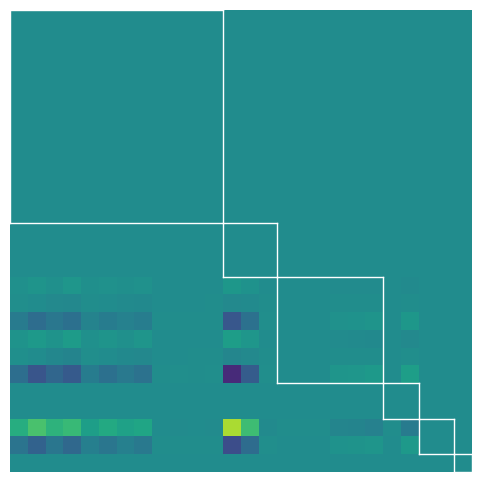
\includegraphics[width=0.22\linewidth]{kfac_pinns_exp/exp04_gramian_contributions/fig/gram_grad_input_output.png}
    &
      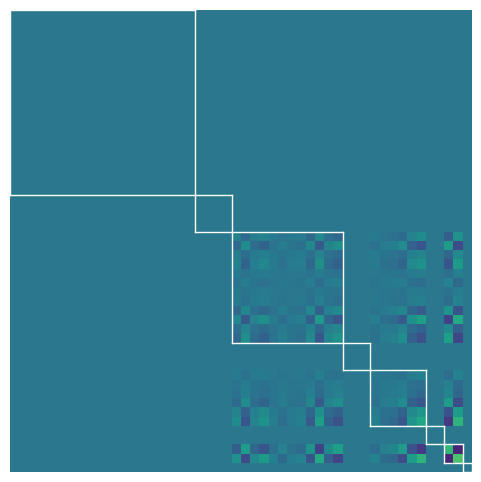
\includegraphics[width=0.22\linewidth]{kfac_pinns_exp/exp04_gramian_contributions/fig/gram_grad_input_grad_input.png}
    &
      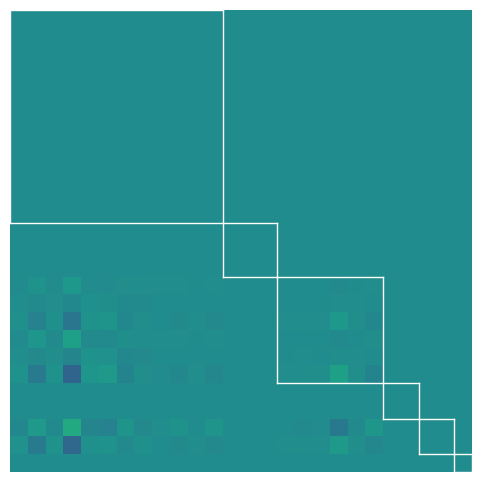
\includegraphics[width=0.22\linewidth]{kfac_pinns_exp/exp04_gramian_contributions/fig/gram_grad_input_hess_input.png}
    \\
    (\textcolor{blue}{Hessian}, \textcolor{red}{forward})
    &
      (\textcolor{blue}{Hessian}, \textcolor{red}{gradient})
    &
      (\textcolor{blue}{Hessian}, \textcolor{red}{Hessian})
    \\
    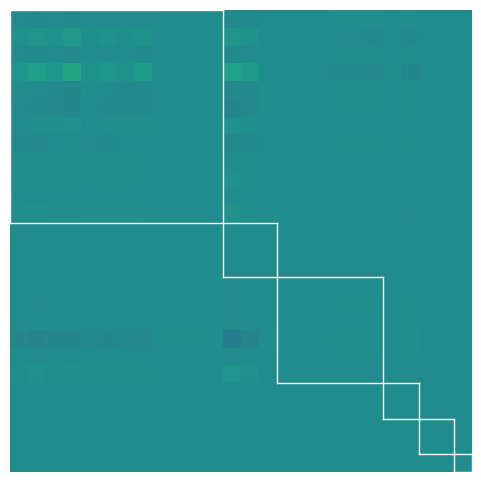
\includegraphics[width=0.22\linewidth]{kfac_pinns_exp/exp04_gramian_contributions/fig/gram_hess_input_output.png}
    &
      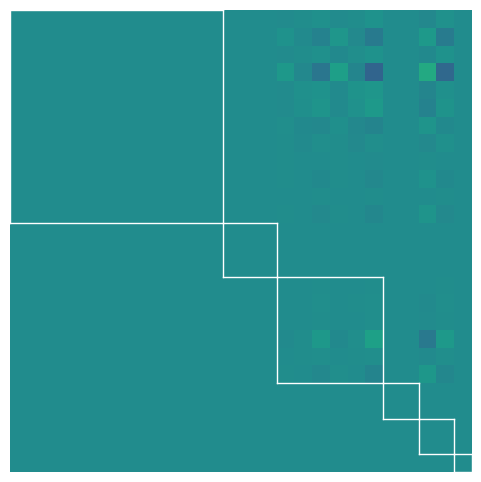
\includegraphics[width=0.22\linewidth]{kfac_pinns_exp/exp04_gramian_contributions/fig/gram_hess_input_grad_input.png}
    &
      
\includegraphics[width=0.22\linewidth]{kfac_pinns_exp/exp04_gramian_contributions/fig/gram_hess_input_hess_input.png}
  \end{tabular}
  \caption{Contributions $\mG_{\Omega,\textcolor{blue}{\bullet}, \textcolor{red}{\bullet}}$ to the Laplacian's Gramian $\mG_{\Omega}$ from different children in the computation graph on a synthetic toy problem.
    We use a $4 \to 3 \to 2 \to 1$ sigmoid-activated MLP and 10 randomly generated inputs. The contributions are highlighted as in \Cref{eq:fisher}.}\label{fig:gramian-contribution-children}
\end{figure}
%%% Local Variables:
%%% mode: latex
%%% TeX-master: "../main"
%%% End:
